\documentclass[conference]{IEEEtran}
\usepackage{cite}
\usepackage{amsmath,amssymb}
\usepackage{graphicx}
\usepackage{booktabs}
\usepackage{url}

\title{Quantifying Reliability in Medical Image Classification\\
Using Multi-Factor Trust Metrics}

\author{\IEEEauthorblockN{Kishore S}
\IEEEauthorblockA{Independent Researcher\\
Email: your-email@example.com}}

\begin{document}
\maketitle

\begin{abstract}
Deep learning models for medical image analysis can achieve high discrimination, but clinical deployment requires reliability signals beyond raw confidence. This paper presents an end-to-end trust-aware framework for chest X-ray classification that combines four reliability factors: (i) predictive confidence, (ii) Bayesian epistemic uncertainty via Monte Carlo (MC) Dropout, (iii) calibration quality using Expected Calibration Error (ECE) with temperature scaling, and (iv) ensemble disagreement across independently trained models. A clinically motivated risk prior increases scrutiny for Pneumonia predictions relative to Normal predictions. These factors are combined into a unified multi-factor trust score and mapped into actionable categories: Reliable, Review Needed, and High Uncertainty. On the Chest X-ray Pneumonia dataset, the framework achieved Accuracy 0.8590, AUC 0.9273, F1 0.8886, ECE reduction from 0.3045 to 0.1844 after temperature scaling, and Brier score 0.1713. A Streamlit dashboard integrates prediction, uncertainty, calibration, disagreement, trust score, and Grad-CAM visual explanations. Results indicate that reliability-aware decision support is more clinically informative than confidence-only reporting.
\end{abstract}

\begin{IEEEkeywords}
Medical AI, Trustworthy AI, Uncertainty Quantification, Calibration, Ensemble Disagreement, Grad-CAM, Chest X-ray
\end{IEEEkeywords}

\section{Introduction}
Deep neural networks have shown strong performance in chest X-ray interpretation and pneumonia detection, with prior studies demonstrating near-radiologist-level discrimination in benchmark settings \cite{rajpurkar2017chexnet}. However, high discrimination alone is insufficient for safe clinical deployment. In practice, decision support systems must communicate when predictions are uncertain, poorly calibrated, or inconsistent across model instances. Overconfident errors in these settings can directly affect downstream triage and treatment decisions.

Recent work highlights two central reliability challenges in modern deep learning: uncertainty estimation and confidence calibration. MC Dropout provides a practical Bayesian approximation for estimating epistemic uncertainty at inference time \cite{gal2016dropout}, while temperature scaling is an effective post-hoc method for reducing confidence miscalibration \cite{guo2017calibration}. Even with these methods, many pipelines still report only a single confidence value, without integrating complementary reliability signals into one actionable indicator for clinicians.

This paper addresses that gap with a multi-factor trust framework for binary chest X-ray classification (Normal vs Pneumonia). Instead of relying on softmax confidence alone, we jointly model predictive confidence, MC Dropout uncertainty, calibration quality (ECE before/after temperature scaling), and ensemble disagreement across independently trained models. We further incorporate class-dependent clinical risk weighting so that higher-risk predictions receive stricter trust scrutiny. The resulting trust score supports transparent triage through interpretable categories: Reliable, Review Needed, and High Uncertainty.

\subsection{Problem Statement}
Given a chest X-ray image $x$, a classifier predicts class probability $p(y\mid x)$ for $y \in \{\text{Normal},\text{Pneumonia}\}$. Existing clinical AI workflows often expose only the maximum softmax probability as confidence, which can be miscalibrated and insensitive to epistemic uncertainty. This creates a safety risk: high-confidence but unreliable predictions may be acted on without sufficient review.

The problem addressed in this work is to design a reliability-aware decision layer that augments classification with actionable trust estimation. Formally, we seek a trust function
\begin{equation}
T(x) = f\big(C(x), U(x), \mathrm{Cal}(x), D(x), R(y)\big),
\end{equation}
where $C$ is calibrated confidence, $U$ is epistemic uncertainty, $\mathrm{Cal}$ represents calibration quality, $D$ is ensemble disagreement, and $R$ is class-dependent clinical risk. The objective is to preserve diagnostic performance while improving decision safety through interpretable trust categories that support triage (Reliable, Review Needed, High Uncertainty).

\textbf{Contributions:}
\begin{itemize}
    \item An end-to-end reliability pipeline built on ResNet18 for chest X-ray classification.
    \item Bayesian uncertainty via MC Dropout with stochastic inference.
    \item Calibration analysis using ECE and temperature scaling.
    \item Ensemble disagreement using three independently trained models.
    \item Risk-aware trust scoring and trust-level categorization for clinical usage.
    \item An interactive dashboard for explainable reliability reporting.
\end{itemize}

\section{Methodology}

\subsection{Base Classifier}
A ResNet18 backbone is used for binary classification (Normal vs Pneumonia). A dropout layer is inserted before the final classifier to support stochastic inference.

\subsection{MC Dropout Uncertainty}
At inference, dropout remains active and each sample is evaluated over $T=30$ stochastic forward passes. Let $p_t$ denote the positive-class probability for pass $t$:
\begin{equation}
\bar{p} = \frac{1}{T}\sum_{t=1}^{T} p_t, \quad
U = \mathrm{Var}(p_t).
\end{equation}
$\bar{p}$ is the mean prediction and $U$ is epistemic uncertainty.

\subsection{Calibration and Temperature Scaling}
Calibration is measured with ECE:
\begin{equation}
\mathrm{ECE} = \sum_{m=1}^{M} \frac{|B_m|}{N} \left|\mathrm{acc}(B_m)-\mathrm{conf}(B_m)\right|,
\end{equation}
where $B_m$ is bin $m$, $\mathrm{acc}(B_m)$ is empirical accuracy, and $\mathrm{conf}(B_m)$ is average confidence. Temperature scaling learns scalar $T_s>0$ on validation logits and uses $z/T_s$ for calibrated inference \cite{guo2017calibration}.

\subsection{Ensemble Disagreement}
Three models with different random seeds are trained. Disagreement for each sample is the variance across model probabilities:
\begin{equation}
D = \mathrm{Var}(p^{(1)}, p^{(2)}, p^{(3)}).
\end{equation}

\subsection{Clinical Risk Weighting and Trust Score}
Risk weights are defined as Normal $=1.0$ and Pneumonia $=1.5$. The final trust score is:
\begin{equation}
\mathrm{Trust} = w_1(1-U) + w_2(1-\mathrm{ECE}) + w_3(1-D) + w_4(C\cdot R),
\end{equation}
where $C$ is calibrated confidence and $R$ is class risk weight. Trust is categorized into Reliable, Review Needed, and High Uncertainty; higher acceptance thresholds are enforced for high-risk predictions.

\section{Experimental Setup}

\subsection{Dataset and Preprocessing}
Experiments use the Chest X-ray Pneumonia dataset. Images are resized to $224\times224$ and normalized with ImageNet statistics. Data augmentation includes random horizontal flip, small rotation, and mild brightness/contrast jitter.

\subsection{Training Protocol}
The model is trained with cross-entropy loss and Adam optimization. Reliability analysis includes 30-pass MC Dropout, 3-model ensemble training, ECE before/after temperature scaling, and validation-optimized decision thresholding.

\subsection{Evaluation Metrics}
We report Accuracy, AUC, F1-score, ECE, Brier score, and average trust score.

\section{Results}

\begin{table}[t]
\caption{Final Evaluation Metrics}
\label{tab:metrics}
\centering
\begin{tabular}{lc}
\toprule
\textbf{Metric} & \textbf{Value} \\
\midrule
Accuracy & 0.8590 \\
AUC & 0.9273 \\
F1-score & 0.8886 \\
ECE (before scaling) & 0.3045 \\
ECE (after scaling) & 0.1844 \\
Brier score & 0.1713 \\
Average trust score & 0.9918 \\
Decision threshold & 0.82 \\
\bottomrule
\end{tabular}
\end{table}

Temperature scaling improves reliability by reducing ECE, indicating confidence calibration gains. The trust score combines complementary reliability factors and enables risk-aware triage.

\begin{figure}[t]
    \centering
    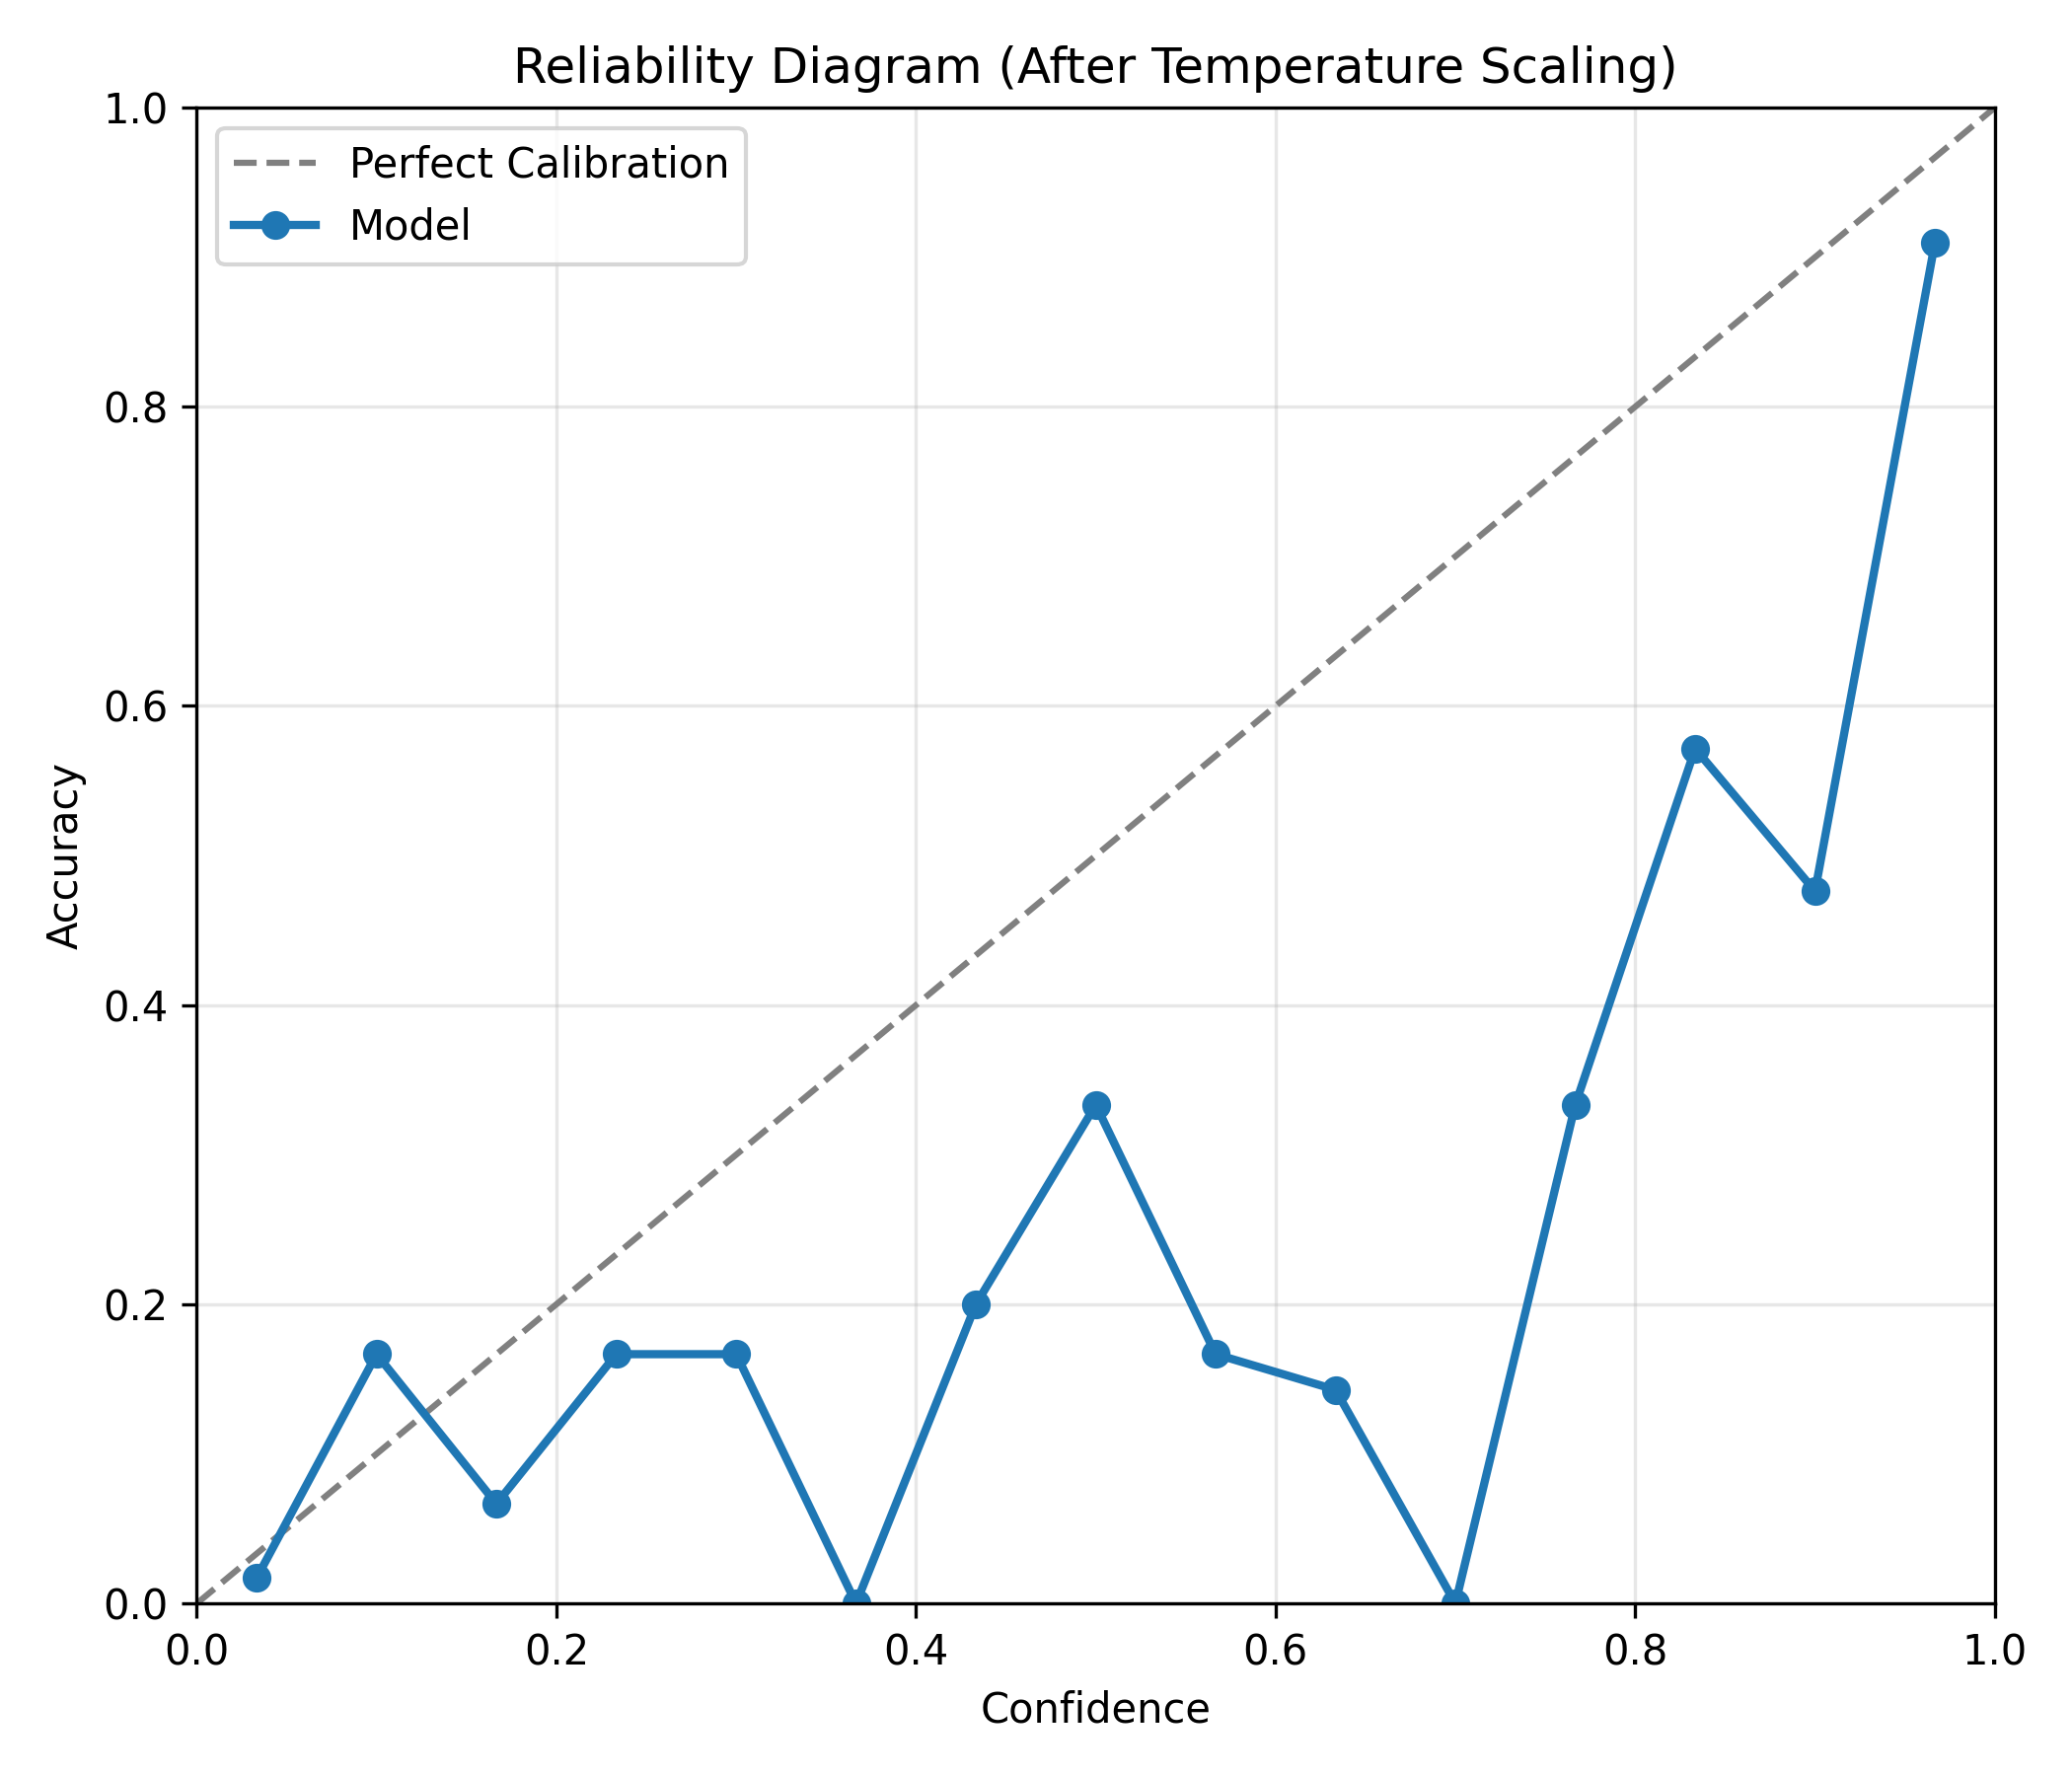
\includegraphics[width=0.95\linewidth]{../artifacts/figures/reliability_after.png}
    \caption{Reliability diagram after temperature scaling.}
    \label{fig:reliability}
\end{figure}

\begin{figure}[t]
    \centering
    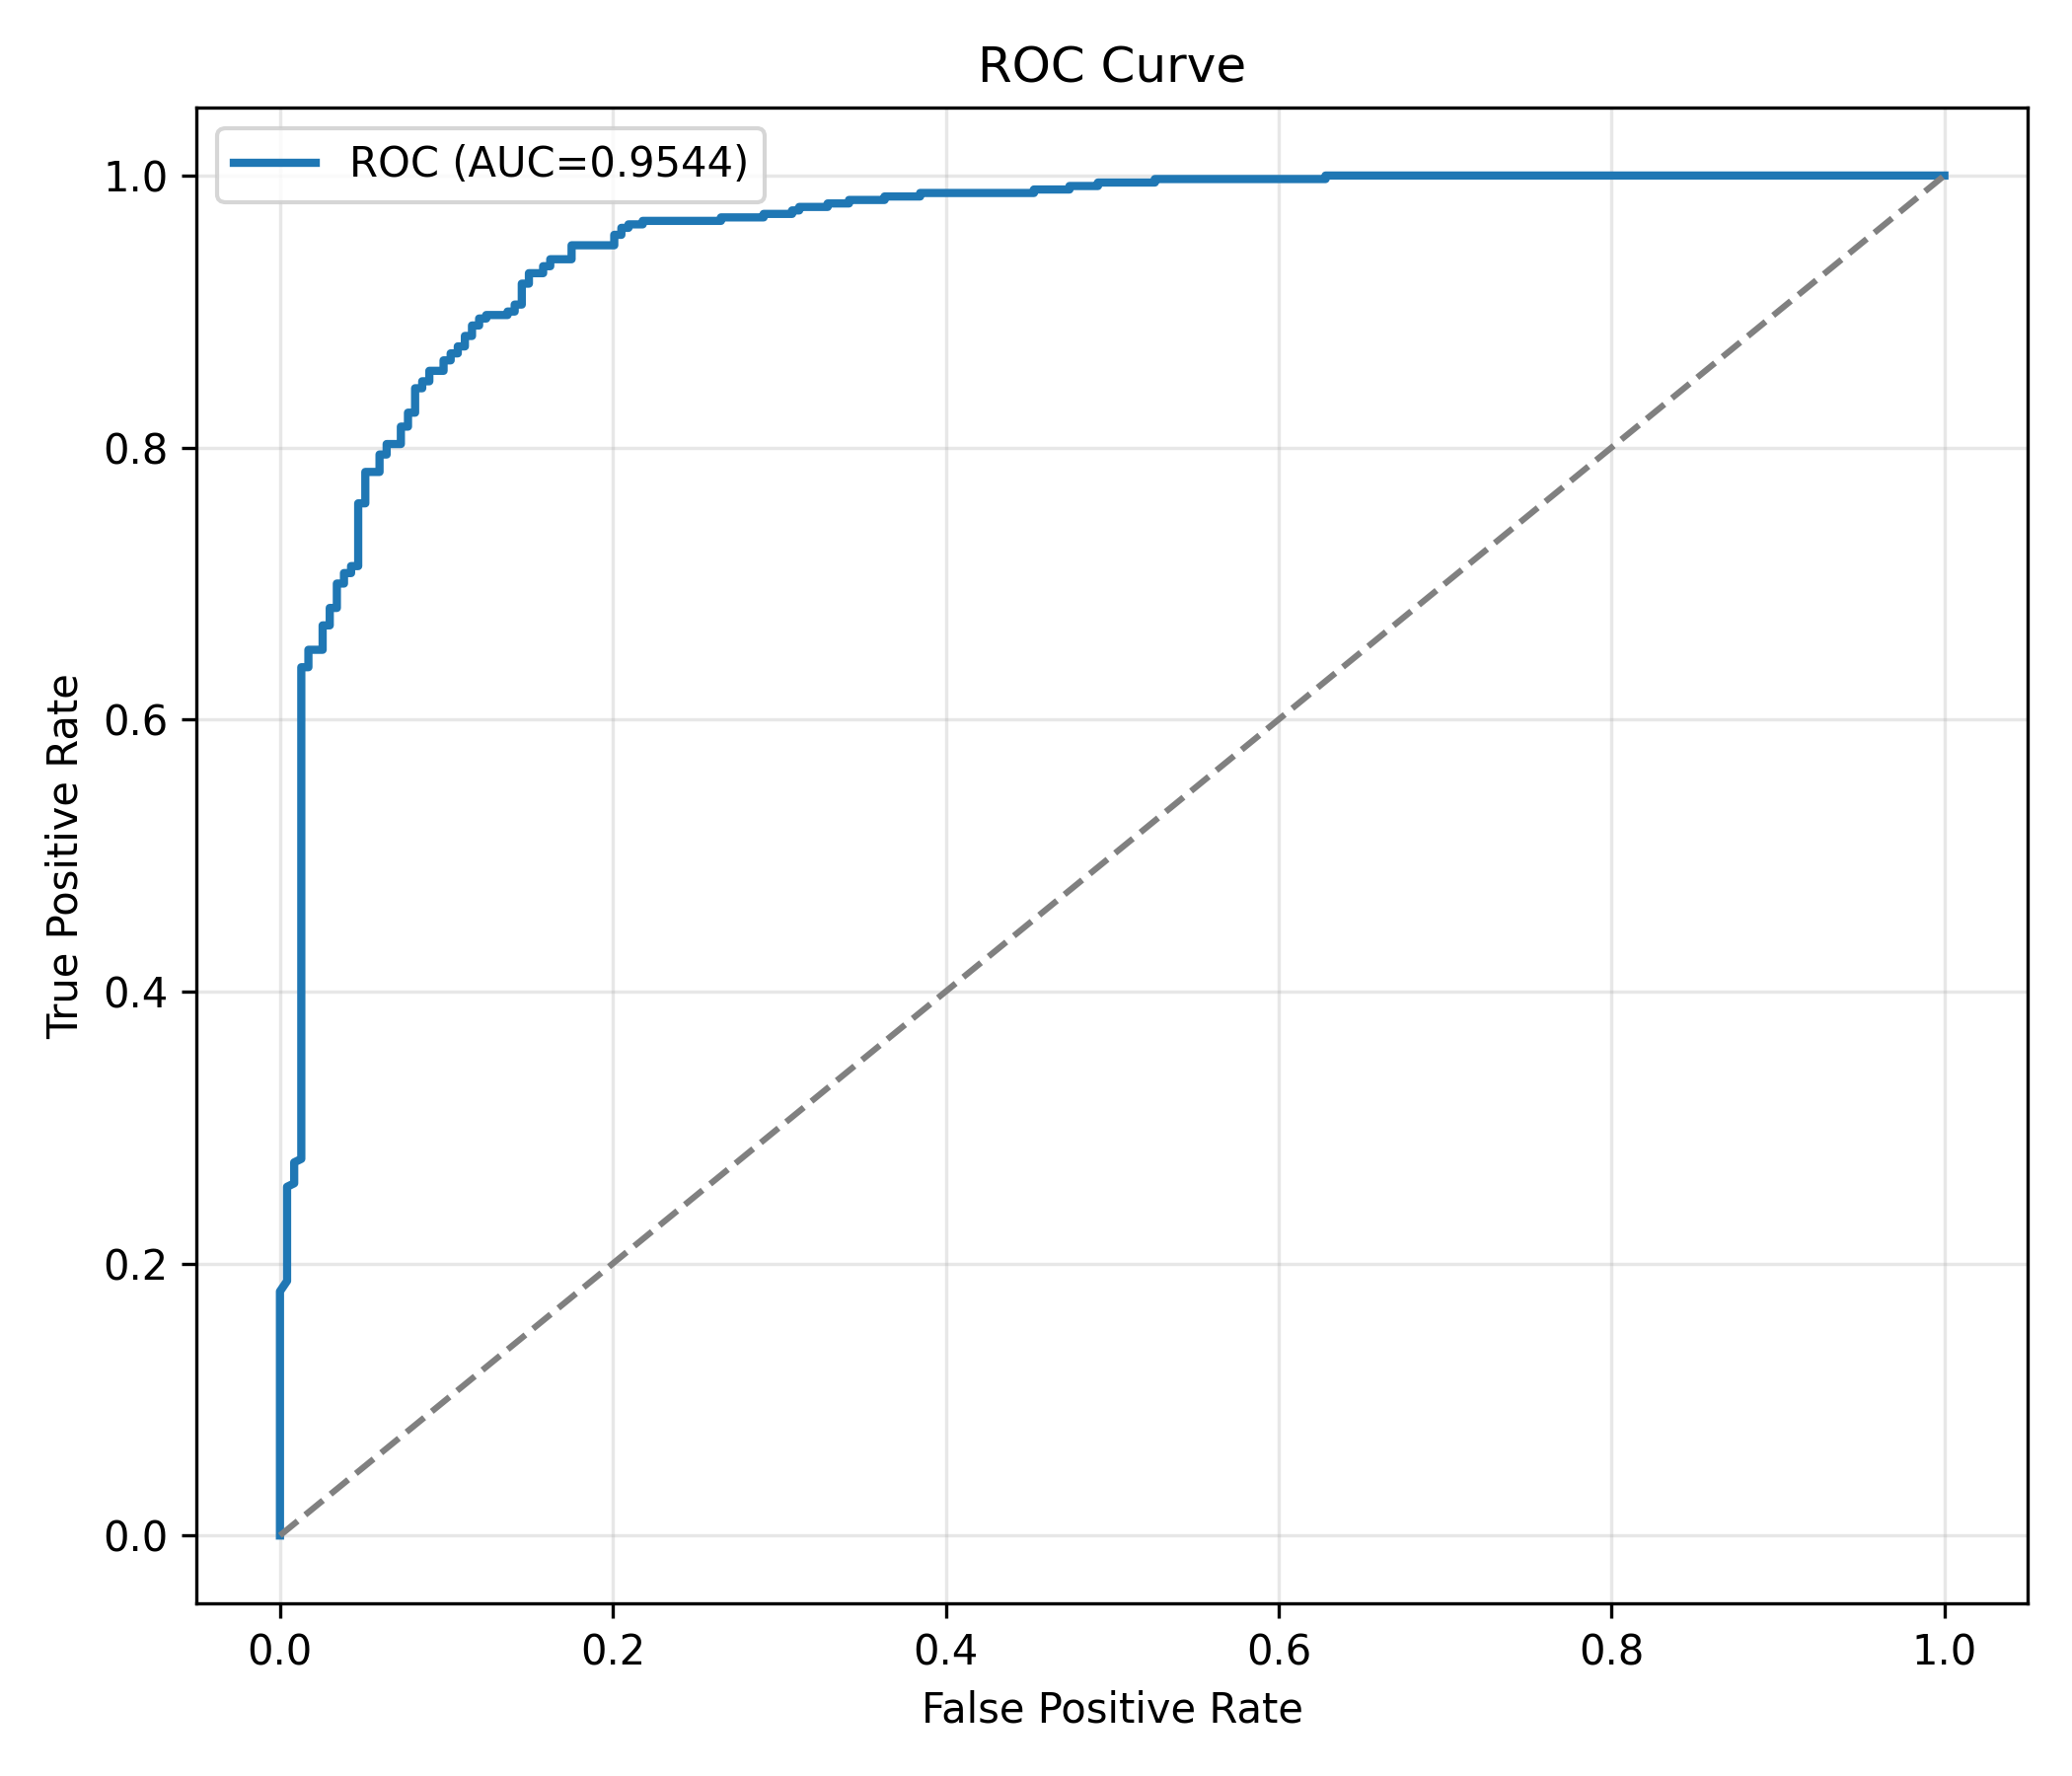
\includegraphics[width=0.95\linewidth]{../artifacts/figures/roc_curve.png}
    \caption{ROC curve for the calibrated classifier.}
    \label{fig:roc}
\end{figure}

\section{Dashboard and Explainability}
A Streamlit dashboard is developed for interactive clinical interpretation. For each uploaded chest X-ray, the interface reports prediction, confidence, MC uncertainty, ECE, ensemble disagreement, trust score gauge, and Grad-CAM heatmap \cite{selvaraju2017gradcam}.

\section{Discussion}
The findings support the view that confidence alone is insufficient for clinical trust. Uncertainty, calibration, and disagreement provide complementary evidence for model reliability. Clinical risk weighting further aligns automated outputs with patient safety priorities by requiring stricter trust criteria for high-risk classes.

\section{Limitations and Future Work}
Current experiments use lightweight training for rapid iteration and a single public dataset. Future work should include longer training schedules, external validation across institutions, out-of-distribution testing, and clinician-calibrated risk thresholds.

\section{Conclusion}
This paper presents a practical and modular framework for reliability-aware medical image classification. By integrating Bayesian uncertainty, calibration, ensemble disagreement, and risk weighting into one trust metric, the system provides transparent and actionable reliability signals for safer deployment.

\bibliographystyle{IEEEtran}
\bibliography{references}

\end{document}
